% Chapter Template

\chapter*{Introduction} % Main chapter title
\addcontentsline{toc}{chapter}{Introduction}
\label{Introduction} % Change X to a consecutive number; for referencing this chapter elsewhere, use \ref{ChapterX}

\lhead{\emph{Introduction}} % Change X to a consecutive number; this is for the header on each page - perhaps a shortened title

\textit{``When you have seen one ant, one bird, one tree, you have not seen them all."}

\begin{flushright}
Edward O. Wilson (1929-.)
\end{flushright}


\cleardoublepage
%----------------------------------------------------------------------------------------
%	SECTION 1
%----------------------------------------------------------------------------------------
\section{La vie en groupe}
\label{sec:vie}

%-----------------------------------
%	SUBSECTION 1
%-----------------------------------

	\subsection{Définition}
    \label{subsec:definitionvie}
Les individus d'une même espèce, ou non, peuvent se réunir et former des groupes sociaux \cite{campan_ethologie._2002}. Il faut distinguer les foules, caractérisées par le rassemblement d'individus recherchant les mêmes conditions écologiques mais n'ayant aucune affinité \cite{campan_ethologie._2002}, des groupes sociaux, caractérisés par la présence de relations privilégiées entre les individus au-delà de la reproduction \cite{campan_ethologie._2002}. On peut ainsi utiliser le terme de \textit{social} dès lors qu'un individu appartient à un groupe social de façon temporaire ou permanente \citep{campan_ethologie._2002, aron_les_2009}.\\
La socialité est présente dans de nombreux taxons animaux (Figure \ref{fig:group}), puisqu'il peut s'agir d'amphibiens, de mammifères ou encore d'arthropodes \citep{campan_ethologie._2002, aron_les_2009}. Ce phénomène polyphylétique est expliquée par cette diversité extrême de taxons. En effet, l'apparition de la vie sociale a, selon \citet{le_masne_classification_1952}, un caractère \textit{sporadique} et \textit{polyphylétique}. Ceci suggérant que les divers types de regroupements sociaux actuels se sont formés d'une manière indépendante, à partir de formes non sociales, au sein de \textit{phyla} bien distincts. Ce phénomène indique par ailleurs que la socialité offre aux individus un avantage évolutif indéniable. Elle constitue une même réponse adaptée d'espèces différentes à des contraintes environnementales.

\begin{figure}[ht]
	\centering
		\includegraphics[width=0.85 \textwidth]{Figures/groupes_pdf.jpg}
		\rule{35em}{0.5pt}
	\caption[Group]{Exemples de regroupements sociaux chez différents taxons animaux. \textbf{A}. Flamants roses, Kenya. \textbf{B}. Raies mantas, Golfe de Californie (photo : F. Schulz). \textbf{C}. Criquets, Madagascar. \textbf{D}. Éléphants, Tchad.}
	\label{fig:group}
\end{figure}

%-----------------------------------
%	SUBSECTION 2
%-----------------------------------

    \subsection{Valeur adaptative et coûts}
    \label{subsec:benef}
A première vue, la vie en groupe apporte des inconvénients. Parmi les plus évidents, on peut citer une transmission facilitée des pathogènes entre les individus ou encore le partage inégal d'une ressource entre les membres d'un groupe social \cite{danchin_ecologie_2005}. Malgré tout, ce mode de vie offre de nombreux bénéfices (recensés par \citet{krause_living_2002}). L'un des plus documenté et étudié dans la littérature est une diminution du risque de prédation \cite{vulinec_collective_1990}. Des effets de dilution/confusion sont notamment impliqués et sont caractérisés par une augmentation soudaine de proies pouvant effrayer le prédateur ou diminuer ses chances de capture. Il y a également une augmentation de la vigilance, l'hypothèse de l'effet \textit{many-eyes}. Plus il y a d'individus, plus il y a d'individus-détecteurs diminuant de fait le temps de détection d'un prédateur. Le regroupement d'individus offre également un rapprochement des partenaires sexuels amenant à une augmentation du taux d'accroissement et de reproduction de la population \cite{courchamp_allee_2008}. Cette liste, bien que non exhaustive, montre certains avantages liés à la vie en groupe. Ces avantages vont être pérennisés par le maintien de la cohésion sociale \cite{krause_living_2002}.
    


%-----------------------------------
%	SUBSECTION 3
%-----------------------------------

    \subsection{Classification}
    \label{subsec:classification}
Plusieurs auteurs se sont essayés à classer les différents niveaux d'organisation sociale. \citet{wheeler_social_1928} fut l'un des précurseurs, et c'est à partir de ses observations sur les insectes qu'il classa les niveaux de socialité sur la base du lien entre la mère et sa progéniture. C'est à partir des travaux de Wheeler que Michener, aidé par Wilson, établit une classification hiérarchique des niveaux de socialité (Tableau \ref{tab:classification}). Cette classification, appelée \textit{classification de Michener-Wilson}, reste à ce jour la plus communément utilisée, et notamment en entomologie. Michener et Wilson considèrent une espèce dite \textit{sociale}, comme toute espèce présentant \textit{une communication réciproque de nature coopérative} \citep{michener_social_1974, wilson_insect_1971}. Par communication est entendue ici \textit{toute action individuelle qui influence la probabilité d'apparition d'un comportement chez un autre individu}. Pour résumer, l'eusocialité caractérise le niveau le plus élevé, que l'on retrouve très majoritairement chez les arthropods et notamment les fourmis, les abeilles ou les termites. Ce stade est défini par un chevauchement des générations d'adultes, une coopération pour les soins aux jeunes et une spécialisation d'individus pour la reproduction (Tableau \ref{tab:classification})


\begin{table}[p]
	\caption[Classification]{Classification des différents niveaux de socialité selon Michener et Wilson (cité dans \citet{lihoreau_organisation_2009} et modifié d'après \citet{aron_les_2009}).}
    \centering
	\includegraphics[width=1 \textwidth]{Figures/classification.png}
		\label{tab:classification}
\end{table}   

\begin{table}[p]
	\caption[Classification2]{Classification des différents niveaux de socialité suite à l'observation des sociétés de vertébrés (tiré de \citet{kerth_group_2010}).}
    \centering
	\includegraphics[width=0.8 \textwidth]{Figures/classification2.png}
		\label{tab:classification2}
\end{table}      

Bien que critiquée par plusieurs auteurs (critiques résumées par \citet{costa_other_2006}), la classification de Michener-Wilson est largement utilisée dans la littérature scientifique. Une critique fréquente est que ces auteurs se sont basés sur des espèces d'arthropodes, et qu'il était donc difficile de transposer cette classification aux sociétés de vertébrés. Une autre classification tirée de l'observation des groupes de vertébrés a été proposée (Tableau \ref{tab:classification2}; \cite{kerth_group_2010}). Avec cette dernière, les groupes de blattes, les volées d'oiseaux ou encore les larves nécrophages de Diptères sont considérées comme \textit{grégaires}. Des exemples de sociétés de type fission/fusion sont retrouvés chez les éléphants (Figure \ref{fig:group}) ou les dauphins. 

Afin d'éviter toute confusion, les termes de \textit{grégaire}, \textit{social} et \textit{eusocial} seront ici utilisés pour définir les niveaux de socialité, en accord avec la classification de Michener-Wilson.
    
  

%----------------------------------------------------------------------------------------
%	SECTION 2
%----------------------------------------------------------------------------------------
\section{L'agrégation}
\label{sec:agregation}
Le comportement d'agrégation, ou grégarisme, est considéré d'un point de vu évolutif comme le premiers pas vers des niveaux de socialité supérieurs \citep{campan_ethologie._2002, aron_les_2009}. Ce comportement d'inter-attraction entre les individus est indépendant de l'attraction sexuelle. Si on se réfère à la distribution spatiale des organismes, \citet{camazine_self-organization_2001} définissent une agrégation comme un assemblage d'individus qui entraîne une forte densité de ceux-ci dans les environs. Ces groupes trouvent leur origine et leur cohésion par l'inter-attraction de leurs membres, d'où la nécessité qu'il y ait un transfert d'information (i.e. communication) entre les individus constituant ce groupe \citep{camazine_self-organization_2001, ame_collegial_2006}. L'agrégation est généralisée aux sociétés d'invertébrés (Figure \ref{fig:aggregation}) et peut apparaître comme une réponse à des hétérogénéités environnementales (agrégation non sociale) ou à l'attraction entre individus (agrégation sociale \cite{costa_other_2006}). Le grégarisme est l'un des phénomènes sociaux les plus primaires, et beaucoup d'activités d'insectes sociaux lui sont liées, comme les déplacements ou le fourragement \citep{deneubourg_dynamics_2002, simpson_gregarious_2001, wertheim_effects_2006}.


%-----------------------------------
%	SUBSECTION 1
%-----------------------------------

    \subsection{Les différents types d'agrégation}
    \label{subsec:types}
Deux types d'agrégation sont classiquement connus et admis dans la littérature: l'agrégation dite \textit{non sociale} et celle dite \textit{sociale}.

L'agrégation non sociale, ou agrégation résultant de l'habitat selon \citet{danchin_evolution_1997}, n'est qu'apparente car elle est dépendante des facteurs abiotiques. Les individus vont répondre positivement à des hétérogénéités environnementales. Imaginons un habitat où on observe un grand nombre de parcelles pauvres et quelques parcelles riches, et qu'une population répartie de manière \textit{libre idéale} s'y trouve. Libre étant défini par le fait que les individus se déplacent entre les diverses parcelles sans aucun coût ni contraintes et idéale mentionne qu'ils connaissent parfaitement l'environnement. Bien qu'il y ait un rassemblement sur les parcelles riches, cette observation ne fait que refléter la variation de la qualité de l'environnement. Il résulte de la somme des réponses individuelles aux hétérogénéités du milieu. Ces caractéristiques du milieu peuvent jouer un rôle de \textit{template}, un modèle, permettant de prédire le pattern agrégatif final observé \cite{camazine_self-organization_2001}.
Un second exemple d'agrégation non sociale apparaît lorsque les facteurs abiotiques vont déplacer et restreindre les individus dans une zone. Les agrégats de méduses en sont un bon exemple. Par la force des courants marins et des vents en surface, des mouvements de convection amènent à la formation d'agrégats contenant de nombreux individus \cite{hamner_regularly_1986}. 

L'agrégation sociale, qui nous intéresse plus particulièrement dans ce travail, est définie par \citet{vulinec_collective_1990} comme étant \textit{la tendance qu'à un animal à s'agréger avec d'autres de façon à ce qu'il soit en contact l'un de l'autre, ou proche, et que la distribution de ces animaux dans l'environnement local soit extrêmement inégale}\footnotemark[1]\footnotetext[1]{\textit{"the tendency of an animal to aggregate with others such that the animals are in contact with one another, or are nearly so, and that the distribution of the animals in the local environment is extremely patchy}" \cite{vulinec_collective_1990}.}. La constitution de ces groupes implique la présence d'interactions sociales \cite{parrish_animal_1997} à plus ou moins longue portée et basées sur des signaux chimiques, visuels, tactiles ou sonores. Ces agrégations sont variables en terme de durées et de compositions. Des espèces peuvent être regroupées durant toute leur vie, comme les fourmis ou les abeilles, ou seulement à un moment de leur développement comme les larves de Diptères. D'autres exemples de grégarisme chez les arthropodes sont présentés dans l'article de vulgarisation paru dans \textit{Espèces} (cf. Annexe \ref{Annexes2}) co-écrit avec Pierre \textsc{Broly} (Unité d'Ecologie Sociale, ULB).


 \begin{figure}[ht]
	\centering
		\includegraphics[width=0.9 \textwidth]{Figures/aggregation.png}
		\rule{35em}{0.5pt}
	\caption[Aggregation]{Exemples d'agrégation chez différents taxons d'arthropodes. \textbf{A}. Bernard l'hermite fraise (\textit{Oenobita perlatus} ; photo : K. Marks). \textbf{B}. Cloportes (\textit{Porcelio scaber} ; photo : S. Reekie). \textbf{C}. Larves nécrophages de Diptères (Calliphoridae ; photo : J. Boulay). \textbf{D}. Chenilles du papillon Ruby-spotted Swallowtail (\textit{Papilio anchisiades} ; photo : V. Ciau). \textbf{E}. Coccinelles (\textit{Harmonia axyridis} ; photo : J. Goddard).}
	\label{fig:aggregation}

\end{figure}


%----------------------------------------------------------------------------------------
%	SECTION 3
%----------------------------------------------------------------------------------------

	\section{L'auto-organisation: de l'individuel au collectif}
    \label{sec:autoorganisation}
La notion d'auto-organisation est appliquée en éthologie, en particulier aux insectes sociaux, pour montrer comment un comportement collectif complexe peut émerger à partir d'interactions simples entre individus (Figure \ref{fig:selforga}; \cite{camazine_self-organization_2001}). \citet{bonabeau_auto-organisation_1997} définissent l'auto-organisation comme \textit{les phénomènes au cours desquels une certaine structuration spatiale et/ou temporelle s'opère plus ou moins "spontanément", ou encore sous l'effet d'un flux énergétique, entropique ou matériel}. Cette définition étant issue de la physique \cite{bonabeau_self-organization_1997}, \citet{camazine_self-organization_2001} en distinguent deux grandes différences avec l'auto-organisation appliquée aux systèmes biologiques. La première est la grande complexité des sous-unités des systèmes biologiques. Les sous-unités en physique sont des objets inanimés alors qu'en biologie se sont des organismes vivants complexes. La seconde concerne la nature des lois qui gouvernent les interactions dans ces deux disciplines. Dans les systèmes physico-chimiques, les patterns créés au travers des interactions obéissent uniquement aux lois de la physique. Les systèmes biologiques obéissent également à ces mêmes lois mais les interactions physiologiques et comportementales sont influencées par les propriétés génétiquement contrôlées des composants. \citet{bonabeau_auto-organisation_1997} précisent cette définition dans le cadre des comportements collectifs comme tout \textit{processus au cours duquel des structures émergent au niveau collectif, à partir de la multitude des interactions entre individus, sans être codées explicitement au niveau individuel}. Ces derniers résument l'auto-organisation à trois points essentiels : \textit{(i) l'apparition d'une structure spatio-temporelle ; (ii) cette structure est principalement produite de l'intérieur du système [...] ; (iii) enfin, la notion mal définie qu'une structure "remarquable" "émerge" est traduite par la difficulté voire l'impossibilité pour un observateur [...] de prédire l'apparition de la structure et encore moins ses propriétés}. 

Derrière cette définition, il vient à l'esprit la notion de \textit{complexité} chère à Edgar Morin \cite{morin_methode_1977}. Sumpter \cite{sumpter_principles_2006} relie cette notion à l'auto-organisation avec cette définition : \textit{Le principe central de l'auto-organisation est que les interactions simples répétées entre les individus peuvent produire des modèles adaptatifs complexes au niveau du groupe}\footnotemark[2].\footnotetext[2]{\textit{"The central tenet of self-organization is that simple repeated interactions between individuals can produce complex adaptive patterns at the level of the group."}\cite{sumpter_principles_2006}}  
Dans sa thèse d'HDR, Gautrais \cite{gautrais_dynamiques_2015} critique l'idée que les interactions entre les individus doivent être \textit{simples} tant qu'elles sont \textit{répétées}. Il liste un certains nombre d'exemples d'interactions, allant des réactions chimiques d'oxydo-réduction aux comportements individuels lors de la construction de pistes chez les fourmis, montrant que ces comportements non rien de "simples". Il avance plutôt l'idée que la multitude d'individus présents se comportent de manière \textit{stochastique} et donc non déterministe. Cet élément offre une source de fluctuation qui constitue l'auto-organisation \cite{gautrais_dynamiques_2015}. Gautrais \cite{gautrais_dynamiques_2015} montre également l'importance de \textit{l'amplification} des interactions plus que leur répétition. Il donne ainsi sa propre définition de l'auto-organisation: \textit{"Modèle expliquant le comportement d’ensemble d’un système stochastique par la possibilité que ses fluctuations aléatoires soient amplifiées."}\cite{gautrais_dynamiques_2015}.
Avec cette dernière définition, on voit bien les deux notions essentielles qui constituent l'auto-organisation : \textit{la stochasticité} et \textit{l'amplification}.
L'un des exemples les plus explicites traduisant ces deux notions est le suivi de piste chez la fourmi \cite{deneubourg_collective_1989}. Si on laisse à une colonie le choix entre deux branches d'un même pont strictement identiques allant du nid à une ressource alimentaire, les premières fourmis vont choisir aléatoirement l'une des deux branches du pont. Ces fourmis vont laisser un marquage chimique au sol (dépôt de piste) incitant leurs congénères à emprunter cette branche. Ce premier choix de branche s'est fait de manière stochastique mais le choix des fourmis suivantes s'est vu biaisé en faveur du pont marqué. Ces dernières vont à leur tour marquer de leur passage cette branche peu marquée augmentant un peu plus les probabilités que d'autres fourmis empruntent cette branche du pont. Cet exemple reflète très bien la dynamique de type amplification d'un système stochastique.

 \begin{figure}[ht]
	\centering
		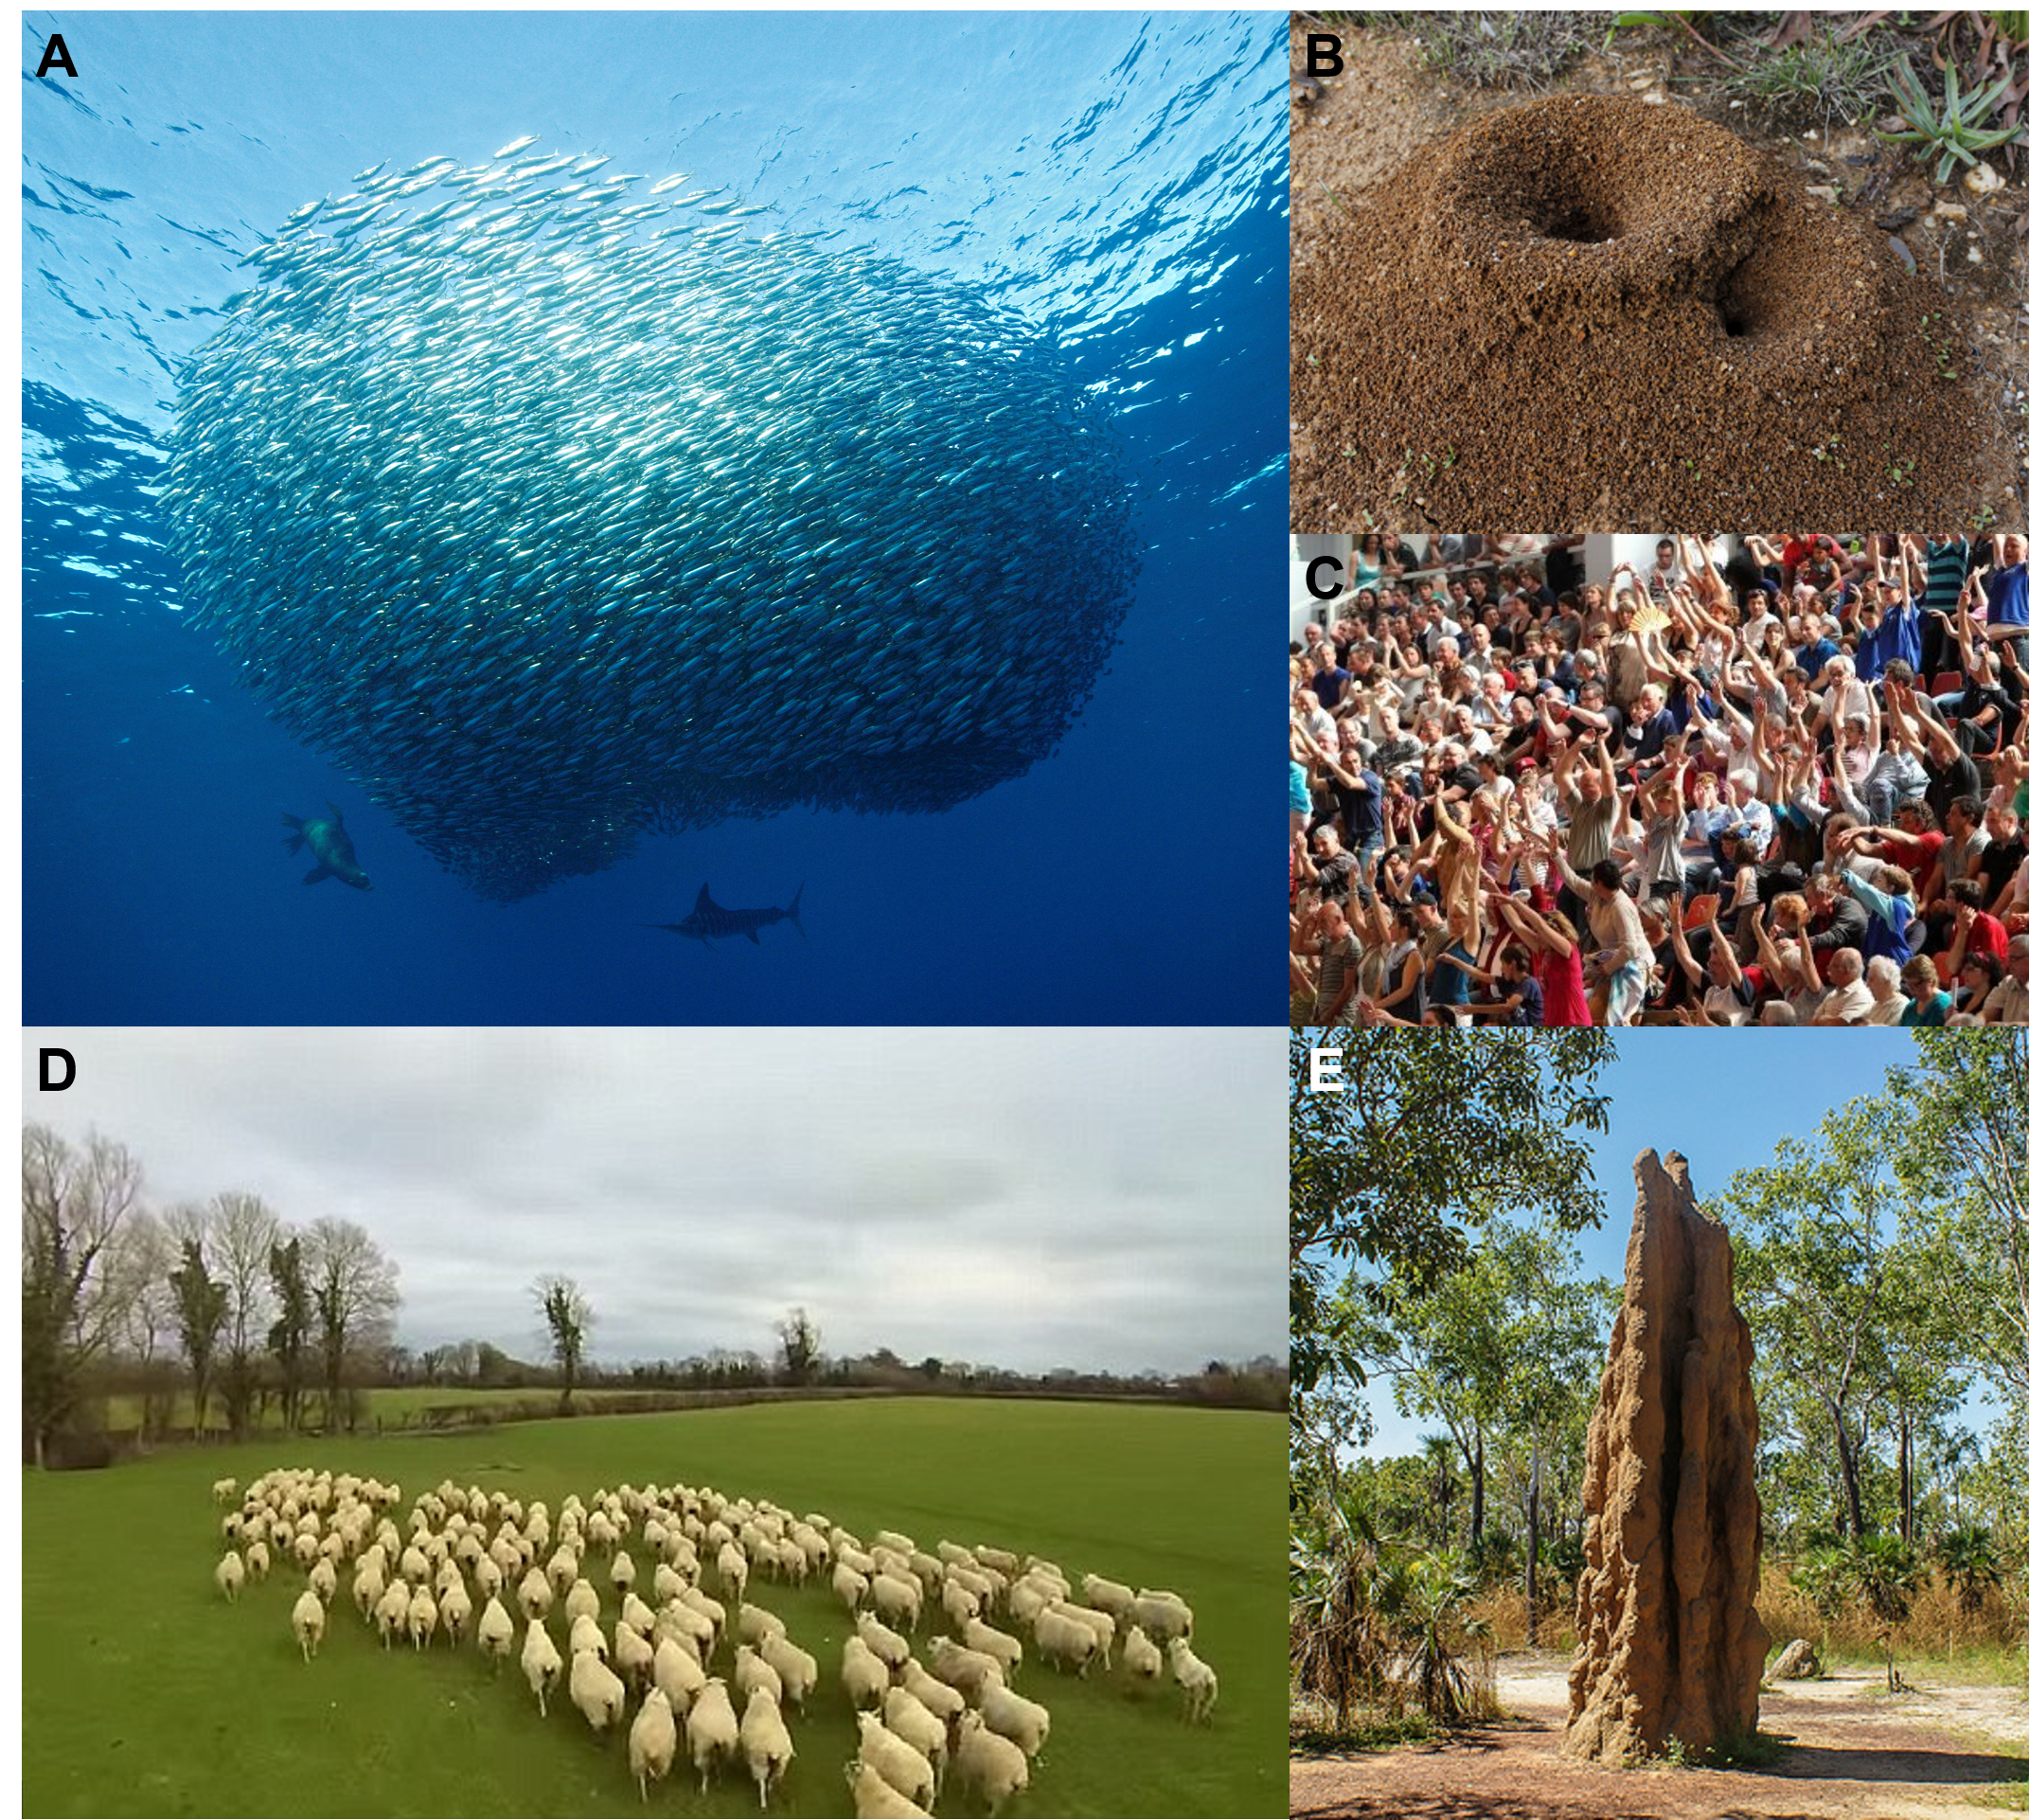
\includegraphics[width=0.8 \textwidth]{Figures/selforga.jpg}
		\rule{35em}{0.5pt}
	\caption[Selforga]{Exemples de structures collectives. \textbf{A}. Banc de sardines (photo: B. Cole). \textbf{B}. Entrée d'un nid de fourmis (\textit{Myrmecia sp.} ; photo : G. Park). \textbf{C}. Mouvement de "Ola" lors d'un match de basketball (photo : Journal Sud Ouest). \textbf{D}. Déplacement collectifs de moutons en Irlande (photo : P. Brennan). \textbf{E}. Nid de termites dans le parc national Litchfield (photo : H. Zaher).}
	\label{fig:selforga}

\end{figure}

%----------------------------------------------------------------------------------------
%	SECTION 4
%----------------------------------------------------------------------------------------

	\section{L'amplification du système}
    \label{sec:amplification}

L'agrégation est une source d'amplification. Une augmentation de la densité d'individus dans une zone accroît de fait la probabilité qu'ont les individus de reproduire une action donnée. Ces mécanismes amplificateurs jouent un rôle déterminant dans l'élaboration des agrégations sociales reposant sur des dynamiques non linéaires \citep{camazine_self-organization_2001, deneubourg_dynamics_2002}.\\  
L'amplification est régie par des boucles rétroactives positives et/ou négatives, appelées \textit{feedbacks}, qui permettent l'accroissement du système mais aussi l'empêchent d'exploser. Un exemple bien connu de feedback positif est le suivi de piste chez les fourmis décrit précédemment (Figure \ref{fig:feedback}). Une fourrageuse dépose une piste chimique allant de la ressource au nid. Ses congénères vont suivre cette piste accroissant sa concentration et ainsi mécaniquement la probabilité que d'autres fourmis suivent cette piste augmente \cite{dussutour_organisation_2004}. Un autre exemple, toujours chez la fourmi, est la probabilité de déposer un cadavre d'une congénères, qui va augmenter avec le nombre de cadavres déjà présents \cite{deneubourg_collective_1989}. La probabilité de quitter un groupe, qui décroit avec le nombre de membres, est un exemple de feedback négatif (Figure \ref{fig:feedback}). A noter qu'avec cet exemple de feedback négatif pairs cela conduit à l'apparition d'un feedback positif (plus d'individus sortent d'un groupe, plus d'individus rejoignent un second groupe). D'autres exemples de feedbacks sont décrits par \citet{jeanson_positive_2009}.\\



 \begin{figure}[ht]
	\centering
		\includegraphics[width=0.9 \textwidth]{Figures/feedback.png}
		\rule{35em}{0.5pt}
	\caption[Feedback]{Exemples de boucles rétroactive positives (+) chez les fourmis et négatives (-) chez les blattes (tiré de \citet{jeanson_positive_2009}).}
	\label{fig:feedback}   
 \end{figure}   
 
%----------------------------------------------------------------------------------------
%	SECTION 5
%----------------------------------------------------------------------------------------
	\section{La prise de décision collective}
    \label{sec:decision}
La prise de décision collective, \textit{collective decision-making}, joue un rôle central dans la vie des animaux sociaux. Les humains en sont un bon exemple avec les élections dans les démocraties. Selon \citet{conradt_consensus_2005} cette décision, souvent appelé abusivement \textit{l'intelligence collective} par le grand public, peut être de deux formes. La première est la \textit{combined decision}, que \citet{conradt_consensus_2005} définissent comme \textit{un choix individuel des membres du groupe (mais pas nécessairement indépendamment) entre deux ou plusieurs actions. Ils ne visent pas un consensus mais les résultats combinés de leurs décisions affectent généralement le groupe dans son ensemble}\footnotemark[3]. Ces auteurs présentent quelques exemples de telles décisions comme l'allocation de tâches chez les insectes eusociaux ou des décisions liées à la consommation chez l'humain. L'individu choisit seul sans chercher un consensus mais son comportement est dépendant de celui du groupe auquel il appartient.

Le second type de décision collective, celui qui nous intéresse dans ce travail, est la décision consensuelle, \textit{consensus decision}, (Figure \ref{fig:consensus}) qui apparaît lorsque \textit{les membres d'un groupe choisissent entre deux ou plusieurs actions mutuellement exclusives dans le but spécifique de parvenir à un consensus}\footnotemark[4] \cite{conradt_consensus_2005}. Les exemples avancés par \citet{conradt_consensus_2005} peuvent être la coordination des prédateurs pour l'attaque d'une proie ou encore le choix d'une destination lors d'un trajet. \citet{conradt_consensus_2005} ont ensuite établi une classification des décisions consensuelles (Figure \ref{fig:consensus}) selon qu'il y ait, ou non, un conflit d'intérêt puis la présence d'une communication globale ou locale. Une communication globale étant définie comme une communication simultanée entre tous les membres du groupe, à la différence de celle locale, où seulement les individus proches peuvent communiquer \cite{conradt_consensus_2005}. Dans le cas des larves nécrophages de Diptères, les individus ont une perception limitée de leur environnement, laissant penser à l'existence d'une communication locale des membres au sein du groupe.

 

\footnotetext[3]{\textbf{Combined decision}: members of a group choose individually (but not necessarily independently) between two or more actions. They do not aim for
consensus but the combined results of their decisions usually affect the group
as a whole.}
\footnotetext[4]{\textbf{Consensus decision}: members of a group choose between two or more mutually exclusive actions with the specific aim of reaching a consensus.}

    
 \begin{figure}[ht]
	\centering
		\includegraphics[width=0.8 \textwidth]{Figures/consensusdecision.png}
		\rule{35em}{0.5pt}
	\caption[Consensus]{Vue schématique de la classification actuelle des décisions consensuelles, \textit{consensus decisions} (tiré de \citet{conradt_consensus_2005}).}
	\label{fig:consensus}   
 \end{figure}       

\clearpage
%----------------------------------------------------------------------------------------
%	SECTION 6
%----------------------------------------------------------------------------------------

\section{Les insectes nécrophages}


%-----------------------------------
%	SUBSECTION 1
%-----------------------------------

	\subsection{L'écosystème cadavre et rôle des insectes}
Par définition, le cadavre est une ressource instable et éphémère. Ce biotope, à haute valeur énergétique, apparaît de façon imprédictible, d'où la nécessité pour les espèces nécrophages, i.e. qui se nourrissent des cadavres, de le détecter et de s'y rendre rapidement. C'est un environnement hétérogène avec différentes gammes de températures ainsi que des spots de nourriture à valeur nutritionnelle inégale (e.g. foie, cerveau etc.) \cite{ireland_effects_2006}.

Les insectes nécrophages sont les principaux artisans de la décomposition d'un cadavre \citep{marchenko_medico-legal_1988, payne_summer_1965}. En s'alimentant, ils vont contribuer de manière significative à augmenter la vitesse de dégradation du cadavre (Figure \ref{fig:degradation}, \cite{payne_summer_1965}). On trouve principalement parmi eux des espèces de Diptères et de Coléoptères.   

\begin{figure}[ht]
\centering
		\includegraphics[width=0.85 \textwidth]{Figures/degradation.png}
		\rule{35em}{0.5pt}
		\caption[Degradation]{Évolution temporelle de la masse de porcelets (\textit{Sus scrofa}) en présence \textbf{A} et en absence \textbf{B} d'insectes nécrophages (tiré de \citet{payne_summer_1965}).}
	\label{fig:degradation}
\end{figure}


%-----------------------------------
%	SUBSECTION 2
%-----------------------------------

    \subsection{Les insectes pionniers : les Diptères Calliphoridae et Sarcophagidae}
Les insectes pionniers que l'on retrouve sur les cadavres en décomposition appartiennent principalement aux Calliphoridae et Sarcophagidae. Ces insectes sont dotés d'organes sensoriels très sensibles leurs permettant de détecter un corps à plusieurs kilomètres de distance \cite{barton_browne_role_1960}. Cette détection se fait dès quelques heures après la mort via la perception des composés volatils relargués par le cadavre \cite{frederickx_responses_2012}. Le cadavre va servir de substrat de ponte et de ressource alimentaire pour leurs larves, appelées couramment asticots.

		\subsubsection{Cycle de développement}
Les Diptères nécrophages sont des insectes holométaboles, c'est-à-dire à métamorphose complète. Leur cycle de développement est composé de 4 stades : œuf, larve, pupe et adulte (Figure \ref{fig:cycle}). La durée de ce cycle est dépendante de deux paramètres : l'espèce et la température. Plus la température ambiante est élevée, plus la durée du cycle de développement est courte (et inversement). De plus, à température identique, des individus vont se développer plus ou moins rapidement selon l'espèce à laquelle ils appartiennent.

La femelle pond ses œufs, préférentiellement au niveau des orifices naturels du corps (Figure \ref{fig:pontes}). Ces œufs sont pondus en paquets d'environ 200 et sont généralement agrégés avec ceux d'autres femelles \citep{fenton_oviposition_1999, brodie_is_2014}. Cette agrégation des pontes est la résultante de signaux attractifs comme la présence d'œufs, de larves et/ou d'adultes. Les femelles vont chercher un site de ponte à la fois humide, évitant ainsi la dessiccation des larves, et permettant pour leur progéniture un accès facile à la nourriture.
Après l'éclosion, les larves vont passer par trois stades (L1, L2 et L3) entrecoupés par deux mues. Puis, le stade pré-pupe, qui est un stade intermédiaire entre L3 et pupe, et qui correspond, chez la plupart des espèces, à la phase d'éloignement du corps. Ensuite, la larve pré-pupe se transforme en pupe (i.e. cocon), d'où émergera un imago (Figure \ref{fig:cycle}).   

\begin{figure}[ht]
\centering
		\includegraphics[width=0.6 \textwidth]{Figures/cycle_d_veloppement.png}
		\rule{35em}{0.5pt}
		\caption[Cycle]{Cycle de développement des Diptères Calliphoridae (schéma : J. Boulay ; Infographie: \textit{Espèces}). A 25\up{o}C, la durée de ce cycle pour \textit{Lucilia sericata} est de 13 jours alors que pour \textit{Calliphora vicina} elle est de 17 jours \cite{marchenko_medico-legal_1988}.}
	\label{fig:cycle}
\end{figure}

\begin{figure}[ht]
\centering
		\includegraphics[width=0.8 \textwidth]{Figures/pontes.pdf}
		\rule{35em}{0.5pt}
		\caption[Pontes]{Pontes agrégées de femelles de Diptères Calliphoridae sur un cadavre de porcelet (photo : Edward B. Mondor).}
	\label{fig:pontes}
\end{figure}
 
        \subsubsection{Importance des Diptères en entomologie forensique}
        \label{subsubsec:forensique}
L'entomologie forensique est l'étude des insectes dans le contexte d'enquêtes judiciaires. Les bases de cette science ont été posées par Jean-Pierre Mégnin en 1894 dans son ouvrage \textit{La Faune des cadavres}. Il est le premier à avoir décrit les différentes successions d'insectes nécrophages sur un cadavre, qu'il a appelé \textit{escouades}. Ces travaux ont montré que les Diptères Calliphoridae font parti des premiers insectes à arriver sur le cadavre.

Ces insectes, dont les durées de développement en fonction de l'espèce et de la température sont bien connues, vont permettre de définir une datation du décès \cite{charabidze_insectes_2014}. Cette datation se fait après identification des insectes et connaissant l'historique thermique du lieu où ces espèces se sont développées. 

Avec toutes ces informations, l'expert entomologiste va pouvoir établir une chronologie débutant par l'arrivée des insectes jusqu'à la découverte du corps (Figure \ref{fig:ipm}). Il faut bien garder à l'esprit que l'expert donne un Intervalle Post-Mortem minimum (IPMmin) et non la date effective de la mort. En effet, suivant l'accessibilité du cadavre et les conditions climatiques, les insectes vont mettre un certain temps à arriver et à pondre sur celui-ci. Un corps retrouvé dans les bois sera rapidement colonisé, et donc un IPMmin proche de la date du décès, en comparaison d'un corps retrouvé dans un coffre de voiture. De même, les conditions climatiques comme le froid ou la pluie vont fortement réduire l'activité des insectes \cite{voss_decomposition_2007}.

Les insectes nécrophages peuvent aussi être utilisés comme matrice pour des dosages toxicologiques, on parle alors d'\textit{entomo-toxicologie}. On peut également les utiliser pour détecter des traces de poudre dues à l'utilisation d'une arme à feu. 

A l'heure actuelle, la physiologie de ces insectes est bien connue alors que les études comportementales font défaut. L'importance des Diptères dans le cadre d'expertise renforce l'idée qu'il est nécessaire d'étudier le comportement de ces insectes. Ces recherches comportementales pourraient permettre \textit{in fine} d'affiner les techniques de datation existantes.

\begin{figure}[ht]
\centering
		\includegraphics[width=0.9 \textwidth]{Figures/IPM.png}
		\rule{35em}{0.5pt}
		\caption[IPM]{Chronologie d'une expertise entomologique du décès. Le délai de colonisation va être impacté par l'accessibilité du corps et des conditions climatiques. La partie élevage se fait en laboratoire en conditions de température et de nourriture contrôlées.}
	\label{fig:ipm}
\end{figure}


%-----------------------------------
%	SUBSECTION 3
%-----------------------------------
 
\subsection{Description du modèle biologique}

Cette thèse s'est essentiellement focalisée sur deux espèces de Diptères Calliphoridae, \textit{Lucilia sericata} (Meigen, 1826) et \textit{Calliphora vomitoria} (Linné, 1758) (Figure \ref{fig:mouche}). L'espèce \textit{Calliphora vicina} (Robineau-Desvoidy, 1830) a été utilisée seulement pour une étude (cf. Chapitre \ref{Chapter5}). Ces espèces sont présentes dans toutes les régions tempérées et tropicales du monde. 

\begin{figure}[ht]
	\centering	
        \begin{subfigure}{0.25\textwidth}
			\includegraphics[width=\linewidth]{Figures/210509alf537luciliaw.pdf}
			\caption{\textit{Lucilia sericata}}
				\label{sub:lucilia}
		\end{subfigure}
		\begin{subfigure}{0.265\textwidth}
			\includegraphics[width=\linewidth]{Figures/Calliphora-vomitoria-03.pdf}
			\caption{\textit{Calliphora vomitoria}}
				\label{sub:calliphora}
		\end{subfigure}
        \begin{subfigure}{0.29\textwidth}
			\includegraphics[width=\linewidth]{Figures/vicina.png}
			\caption{\textit{Calliphora vicina}}
				\label{sub:calliphoravic}
		\end{subfigure}
		\rule{35em}{0.5pt}
        \caption[Species]{La mouche verte (\textbf{A}) et les mouches bleues (\textbf{B} et \textbf{C}), les espèces utilisées lors de ce travail.}		
			\label{fig:mouche}
	\end{figure}

    
    \subsubsection{Anatomie}
		\label{subsubsec:anatomie}
Les larves nécrophages de Diptères disposent de deux crochets buccaux antérieurs utilisés pour l'alimentation (Figure \ref{fig:organes}). Dans cette même région, deux organes sensoriels présents en paire sont présents : l'organe dorsal (\textit{Dorsal Organ (DO)}), utilisé pour l'olfaction \cite{chu-wang_fine_1971-1} et l'organe terminal (\textit{Terminal Organ (TO)}) utilisé pour la gustation \cite{chu-wang_fine_1971} (Figure \ref{fig:organes}). Les larves disposent également de 12 photorécepteurs regroupés sous le nom \textit{d'organe de Bolwig} \cite{hinnemann_see_2010}. Cet organe détecte la lumière sur un spectre allant de 400 à 630nm \cite{hinnemann_see_2010}. La Figure \ref{fig:organes} a été obtenue en photographiant une larve L3 de \textit{Lucilia sericata} avec un Microscope Électronique à Balayage Environnemental (MEBE). Cet appareil permet de photographier le sujet sans passer par une étape de métallisation des tissus comme utilisée par \citet{colwell_preparation_1986}.  

Sur la partie postérieure, des stigmates sont présents permettant aux larves de respirer (Figure \ref{fig:stigmates}). L'emplacement, non intuitif pour un humain, de ces stigmates permet aux larves de respirer tout en se nourrissant sur le cadavre. Après chaque mue, une fente s'ajoute à celles déjà présentes (stade L1, stigmate à une fente ; stade L2, stigmates à deux fentes et stade L3, stigmates à trois fentes). Cette caractéristique permet de distinguer facilement le stade de développement de la larve observée.

\begin{figure}[p]
\centering
		\includegraphics[width=0.9 \textwidth]{Figures/organes.png}
		\rule{35em}{0.5pt}
		\caption[Organes]{Organes sensoriels d'une larve de \textit{Lucilia sericata} observés au microscope électronique à balayage environnemental (MEBE). \textbf{A}. Tête de la larve avec la présence des crochets buccaux. \textbf{B}. \textit{Dorsal organ (DO)} utilisé pour l'olfaction. \textbf{C}. \textit{Terminal Organ (TO)} utilisé pour la gustation (photos : J. Boulay avec l'aide de Lucile \textsc{Géant} (Technicienne au Laboratoire d'Analyses Physiques et de Caractérisation des Matériaux, Douai)).}
	\label{fig:organes}
\end{figure}

\begin{figure}[ht]
\centering
		\includegraphics[width=0.7 \textwidth]{Figures/stigmates.png}
		\rule{35em}{0.5pt}
		\caption[Stigmates]{Vue postérieure d’une larve de \textit{Calliphora vicina}
(Diptera : Calliphoridae) au stade L3. Les fentes des stigmates postérieurs permettent de déterminer rapidement le stade de l’individu : 1 fente par stigmate au stade L1, 2 au stade L2 et 3 au stade L3 (photo : B. Bourel).}
	\label{fig:stigmates}
\end{figure}
\clearpage

    \subsubsection{Comportement}
Cette section est issue du Chapitre \textit{Comportement et développement des larves nécrophages} présent dans le livre \textit{Insectes, cadavres et scènes de crime} (Édition: De Boeck ; Éditeurs: D. \textsc{Charabidzé} et M. \textsc{Gosselin}) et écrit en collaboration étroite avec Cindy \textsc{Aubernon} et Damien \textsc{Charabidzé}.


\blockquote{Sur un corps en décomposition, il est fréquent d’observer des masses de larves de Diptères pouvant compter plusieurs centaines à plusieurs milliers d’individus. Les larves qui composent ces masses vont rester en contact physique (agrégat) et se nourrir au même endroit sur le cadavre \cite{rivers_physiological_2011}.}

\blockquote{Du fait de ce comportement grégaire très prononcé, les larves sont en constante bousculade (\textit{scramble competition}) au sein des agrégats. Cette intense activité génère un dégagement de chaleur métabolique pouvant atteindre plusieurs dizaines de degrés (Figure \ref{fig:mass}). Plus la quantité de larve est importante, plus le dégagement de chaleur est élevé \cite{charabidze_larval-mass_2011}. Cette augmentation de température est propice au développement des larves puisqu’elle permet de diminuer sa durée et de ce fait, le temps passé sur le cadavre, limitant ainsi les risques de prédation. Une augmentation trop importante de la température risquerait cependant de tuer les larves. Il existe donc des feedbacks négatifs qui jouent le rôle de régulateurs. Ces régulateurs sont généralement des contraintes physiques et environnementales (Figure \ref{fig:schema}). Chez \textit{L. sericata}, il parait probable que l’accès à la nourriture ainsi que la température locale soient deux facteurs impliqués dans la régulation de la densité et de la localisation des agrégats larvaires \cite{charabidze_larval-mass_2011}.}

\blockquote{Outre le dégagement de chaleur, \citet{rivers_physiological_2011} mettent en avant plusieurs bénéfices liés à l’agrégation (Figure \ref{fig:schema}). Le premier est une coopération pour la digestion. En effet, les larves ont une digestion dite extracorporelle : elles sécrètent une salive riche en antibiotiques et en enzymes protéolytiques qui permettent de liquéfier les tissus \citep{sandeman_tryptic_1990, padilha_sequence_2009}. Plus il y a de larves, plus la quantité de sécrétions salivaires est importante, aboutissant ainsi à une liquéfaction facilitée
des tissus et donc une meilleure assimilation \cite{rivers_physiological_2011}. Un autre bénéfice fréquemment cité est la diminution du risque de prédation. Cette stratégie d’évitement des prédateurs n’a cependant pas été étudiée chez les larves nécrophages de Diptères. Il est enfin probable que l’agrégation limite les pertes d’eau des individus et les protège contre la dessiccation.}

\blockquote{Parallèlement à ces bénéfices, \citet{rivers_physiological_2011}) avancent trois effets délétères majeurs dus à l’agrégation chez les larves de Diptères nécrophages (Figure \ref{fig:schema}. La production de chaleur au sein de l’agrégat peut aboutir à un stress thermique compromettant le développement normal des larves. \citet{wertheim_pheromone-mediated_2005} ont également mis en évidence une chemoattraction des prédateurs et des parasitoïdes, attirés par l’odeur des masses de larves. Enfin, la problématique majeure du grégarisme est la surpopulation au sein des agrégats.
La ponte des femelles étant stimulée par différents signaux attractifs (présence d'œufs, de larves), il y a dans un premier temps agrégation des œufs \cite{esser_factors_1990}. Lorsque les jeunes larves écloses, elles sont donc déjà agrégées sur certaines zones du corps, notamment au niveau des orifices naturels. Au fur et à mesure du développement, la masse larvaire augmente en volume et consomme les ressources. L’appauvrissement des ressources et l’accumulation des déjections (ammoniaque) peut alors compromettre le développement des larves. \citet{kuusela_community_1983} et \citet{prinkkila_complex_1995} démontrent par exemple un effet négatif de la compétition (forte densité larvaire) sur le développement des larves de \textit{Lucilia}. Cependant l’effet contraire, c’est-à-dire une augmentation de la vitesse de développement lorsque la densité augmente, a été décrit chez \textit{Calliphora vicina} \cite{saunders_effects_2013} et \textit{Calliphora vomitoria} \citep{kaneshrajah_calliphora_2004, ireland_effects_2006}. Bien que de tels effets de la densité de larves existent en conditions naturelles et doivent être gardés à l’esprit, il est rare dans un contexte forensique que le cadavre soit une ressource limitante pour les larves de Diptères Calliphoridae. La compétition (hors prédation) est donc généralement faible et n’a alors que peu d’effets sur le développement des larves et l’estimation de l’intervalle post-mortem.}


\begin{figure}[ht]
\centering
		\begin{subfigure}{0.4\textwidth}
			\includegraphics[width=\linewidth]{Figures/mass2.png}
			\caption{Masse larvaire}
				\label{sub:mass2}
		\end{subfigure}
		\begin{subfigure}{0.5\textwidth}
			\includegraphics[width= \textwidth]{Figures/larvalmass.JPG}
			\caption[Larval mass]{Larval-mass effect}
		\end{subfigure}
    \rule{35em}{0.5pt}
    \caption{\textbf{A}. Masse larvaire sur un cadavre de porc (\textit{Sus Scrofa} ; photo : J. Boulay). \textbf{B}. Génération de chaleur au sein d’une masse de larves de Calliphoridae (\textit{larval-mass effect}). Cette augmentation locale de la température est positivement corrélée au nombre d’individus présent au sein de la
masse. Cette chaleur accélère le développement des larves, diminuant ainsi le temps passé sur le cadavre en décomposition (photo : D. Charabidzé).}
    \label{fig:mass}
\end{figure}

\begin{figure}[ht]
\centering
		\includegraphics[width=0.9 \textwidth]{Figures/schema.png}
		\rule{35em}{0.5pt}
		\caption[Schema]{Schéma récapitulatif des bénéfices et des effets
délétères liés à l’agrégation ainsi que des mécanismes permettant l’initiation, l’amplification et la régulation du groupe chez les larves grégaires de Calliphoridae et de Sarcophagidae \\ (schéma: J. Boulay).}
	\label{fig:schema}
\end{figure}

\clearpage